%MCQMC 2012, Sydney
\documentclass[9pt,mathserif]{beamer} %slides and notes
\usepackage{amsmath,booktabs,multirow,natbib,array,minted,graphicx}
%\usepackage{datetime,rotating,bbding,pifont}
\usetheme{FredIIT}
%\usepackage{beamerthemesplit}
\newfont{\hge}{hge scaled 1500}
\newfont{\bighge}{hge scaled 2500}
\newfont{\smallhge}{hge scaled 1200}

\setlength{\parskip}{2ex}

\setlength{\arraycolsep}{0.5ex}

%\logo{\includegraphics[width=0.5cm]{IIT_mark_1c_red.eps}}
\logo{\includegraphics[width=0.5cm]{MengerIITRedGray.eps}}

\title[Adaptive Monte Carlo]{Monte Carlo Algorithms Where the Integrand Size is Unknown}
\author[hickernell@iit.edu]{Fred J. Hickernell}
\institute{\small{Department of Applied Mathematics \\  Illinois Institute of Technology \\
Email: \url{hickernell@iit.edu},
Web: \url{www.iit.edu/~hickernell}\\[3ex]
Joint work with Lan Jiang, Yuewei Liu, and Art Owen\\[3ex]
Thanks to Ian Sloan, Frances Kuo, Josef Dick, and Gareth Peters for inviting me.  \\
This work is partially supported by NSF-DMS-1115392 and NSF-DMS-1135257 grants.}}
\date[MCQMC 2012]{Feb.\ 16, 2012}

%(Quasi-) Monte Carlo algorithms approximate integrals by sample averages.  The error analyses of these algorithms involve measures of the \emph{size} of the integrand, $\sigma(\cdot)$, e.g.,  $\sigma(f) \ge 0$ may denote the standard deviation of $f$ or the variation of $f$. Size measures satisfy $\sigma( cf) = |c| \sigma(f)$.  The number of samples, $n$, needed to ensure that a specified error tolerance, $\varepsilon>0$, is met then depends on $\sigma(f)$, which is typically unknown in advance.  Estimating $\sigma(f)$ numerically turns the original non-adaptive algorithm into an adaptive one while introducing another source of numerical error.
%
%This talk presents an error analysis for numerical integration by (quasi-) Monte Carlo methods that accommodates the need to estimate $\sigma(f)$.  Given $\varepsilon >0$, a practical algorithm is presented that produces an estimate of the integral that is --- absolutely or with high probability --- within $\varepsilon$ of the true value, but without knowing $\sigma(f)$ in a priori.  The cost of this algorithm depends on $\sigma(f)$ as one would expect if $\sigma(f)$ were known in advance. The algorithm presented here is guaranteed provided that the integrand is not too nasty.  The nastiness measure is scale-invariant, i.e., $\text{nasty}(cf) = \text{nasty}(f)$ for $c \ne 0$, and moderate nastiness implies that $\sigma(f)$ can be easily estimated.  For i.i.d.\ sampling, $\text{nasty}(f)$ corresponds to the kurtosis of the integrand.
%

\input FJHDef.tex

\newcommand{\tol}{\text{tol}}
\newcommand{\Pgrid}{P_{\text{grid}}}
\newcommand{\Plat}{P_{\text{lat}}}
\newcommand{\Platdual}{P_{\text{lat}}^{\perp}}
\newcommand{\Pran}{P_{\text{ran}}}
%\newcommand{\cl}{\mathcal{L}}
\DeclareMathOperator{\hatfun}{hat}
\DeclareMathOperator{\cubMC}{cubMC}
\DeclareMathOperator{\qse}{qse}

\def\newblock{\hskip .11em plus .33em minus .07em}

\newcommand{\payoff}{\text{payoff}}
\newcommand{\Eurocallpayoff}{\text{Euro call payoff}}
\newcommand{\Europutpayoff}{\text{Euro put payoff}}
\newcommand{\callpayoff}{\text{call payoff}}
\newcommand{\putpayoff}{\text{put payoff}}

\renewcommand{\d}{{\rm d}}
\DeclareMathOperator{\size}{size}
\DeclareMathOperator{\worst}{worst}
\DeclareMathOperator{\randerr}{rand-err}
\DeclareMathOperator{\worsterr}{worst-err}
\DeclareMathOperator{\worstbias}{worst-bias}
\DeclareMathOperator{\worstvar}{worst-var}
\DeclareMathOperator{\worststd}{worst-std}
\DeclareMathOperator{\Exp}{Exponential}
\DeclareMathOperator{\Gam}{Gamma}
\DeclareMathOperator{\Ber}{Bernoulli}
\DeclareMathOperator{\Bin}{Binomial}
\DeclareMathOperator{\NegBin}{NegBin}
\DeclareMathOperator{\HyperGeo}{HyperGeo}
\DeclareMathOperator{\Pois}{Poisson}
\DeclareMathOperator{\Unif}{Uniform}
\DeclareMathOperator{\MSE}{MSE}
\DeclareMathOperator{\RMSE}{RMSE}
\DeclareMathOperator{\MLE}{MLE}
\DeclareMathOperator{\RR}{RR}
\DeclareMathOperator{\SSTot}{SSTot}
\DeclareMathOperator{\SSTreat}{SSTreat}
\DeclareMathOperator{\SSReg}{SSReg}
\DeclareMathOperator{\SSErr}{SSErr}
\DeclareMathOperator{\MSTreat}{MSTreat}
\DeclareMathOperator{\MSReg}{MSReg}
\DeclareMathOperator{\MSErr}{MSErr}
\DeclareMathOperator{\Poisson}{Poisson}
\DeclareMathOperator{\Student}{Student}
%\DeclareMathOperator{\med}{med}
\DeclareMathOperator{\modee}{mode}
\DeclareMathOperator{\quant}{quant}
\DeclareMathOperator{\eff}{eff}
\DeclareMathOperator*{\argmax}{argmax}
\DeclareMathOperator{\power}{power}
%\DeclareMathOperator{\Pr}{Prob}
\newcommand{\barX}{\bar{X}}
\newcommand{\barx}{\bar{x}}
\newcommand{\barY}{\bar{Y}}
\newcommand{\hatB}{\widehat{B}}
\newcommand{\hatY}{\hat{Y}}
\newcommand{\bary}{\bar{y}}
\newcommand{\barZ}{\bar{Z}}
\newcommand{\hM}{\hat{M}}
%\newcommand{\hmu}{\hat{\mu}}
%\newcommand{\htheta}{\hat{\theta}}
%\newcommand{\hTheta}{\hat{\Theta}}
\newcommand{\hDelta}{\hat{\Delta}}
%\newcommand{\hbeta}{\hat{\beta}}
%\newcommand{\hvbeta}{\hat{\vbeta}}
\newcommand{\barS}{\bar{S}}
\newcommand{\barT}{\bar{T}}
\newcommand{\barr}{\bar{r}}
\newcommand{\barsigma}{\bar{\sigma}}
\newcommand{\geo}{\text{geo}}
\newcommand{\ari}{\text{ari}}
\newcommand{\desn}{\{\vx_i\}_{i=1}^n}
%\newcommand{\ch}{\mathcal{H}}
\newcommand{\fudge}{\mathfrak{C}}


\begin{document}
\frame{\titlepage}

\section{Introduction}

\subsection*{How to Determine Sample Size}

\frame<1-9>[label=converse]{\frametitle{\only<10>{Recall Our }Hypothetical Conversation}
\vspace*{-2ex}
\begin{center}
\begin{tabular}{m{5.5cm}m{5.5cm}} 
Practitioner & You, the Expert \\
\toprule
\uncover<1->{I need to evaluate \alert{integrals}
\[
\mu= \int_{\reals^d} f(\vx) \, \rho(\vx) \, \dif \vx,
\]
for many different $f$, where $\rho$ is a given probability density function.} & 
\uncover<2->{Try a \alert{sample average},
\[
\hmu = \frac 1n \sum_{i=1}^n f(\vX_{i\only<7->{\alert<7>{+n_{\sigma}}}}),
\]
where the $\vX_i$ are i.i.d.\ $\sim \rho$.} \\[2ex]

\uncover<3->{How large should I make \alert{$n$}\only<3-4>{?}\uncover<5->{\ to obtain $\abs{\mu-\hmu} \le \varepsilon$?}} & 
\only<4>{As large as your computational budget allows.}\only<5->{The \alert{Central Limit Theorem} says \[n = \left \lceil \left(\frac{1.96 \only<5-6>{\sigma}\only<7->{\alert<7>{\hsigma}}}{\varepsilon}\right)^2 \right \rceil
\]\only<5-6>{where $\sigma^2$ is the variance of the integrand.}}\\
\uncover<6->{How do I find \alert{$\sigma^2$}?} &
%\vspace*{-1ex}
\uncover<7->{Try the \alert{sample variance} times a \alert{variance inflation factor}:
\[
\hsigma^2 = \frac{\fudge^2}{n_{\sigma}-1} \sum_{i=1}^{n_{\sigma}} [f(\vX_i) - \hmu_{\sigma}]^2.
\]
}\\[-2ex]
\uncover<8->{Does theory \alert{guarantee} that this algorithm works (at least $95\%$ of the time)?} &
\uncover<9->{\alert{Yes!}  This algorithm, with minor modifications, carries a \alert{limited warranty}.}
\end{tabular}
\end{center}
}

\frame{\frametitle{Three Perspectives}
\[
\mu= E[f(\vX)] = \int_{\reals^d} f(\vx) \, \rho(\vx) \, \dif \vx = ?
\]

\begin{description}
\item[Algorithm Design] Construct an automatic multivariate integrator analogous to MATLAB's \alert{\tt quad} for univariate integrals.

\item[Information-Based Complexity] Construct an algorithm, $A$, satisfying $\abs{\mu - A(f)} \le \epsilon$ (definitely, with high probability, or on average)  with $\cost(\varepsilon,A,f)$ depending reasonably on $\varepsilon$ and the \alert{unknown} $\size(f)$.

\item[Statistics] Find a nonparametric confidence interval of \alert{prescribed half-width} $\varepsilon$ for $\mu$ from a reasonable number of samples $Y_i=f(\vX_i)$.

\end{description}
}

\subsection*{MATLAB's {\tt quad} function}

\begin{frame}[fragile]\frametitle{MATLAB's Quadrature Routine {\tt quad} Works Well, \emph{but It Can Be Fooled}}
\begin{tabular}{>{\centering}m{3.7cm}>{\centering}m{3.7cm}>{\centering}m{3.7cm}}
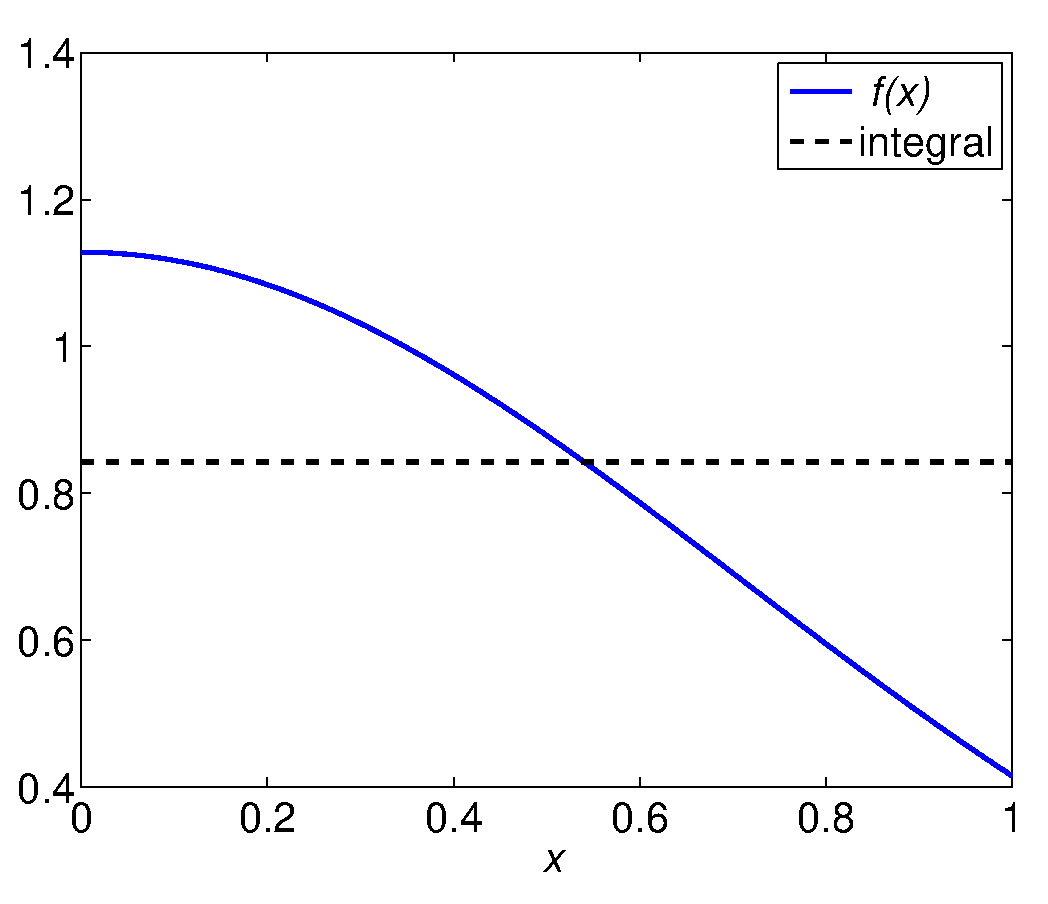
\includegraphics[width=3.7cm]{erfplot.eps}
&
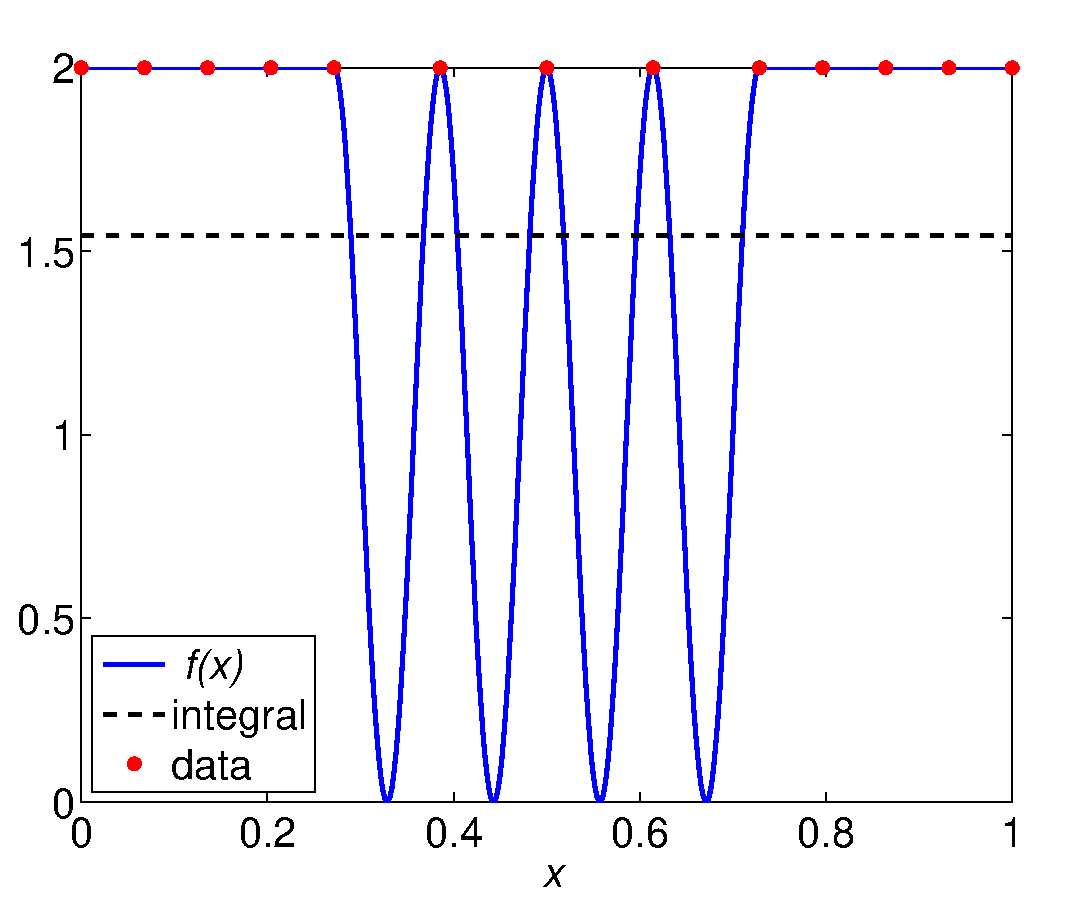
\includegraphics[width=3.7cm]{FoolQuadFunction.eps}
&
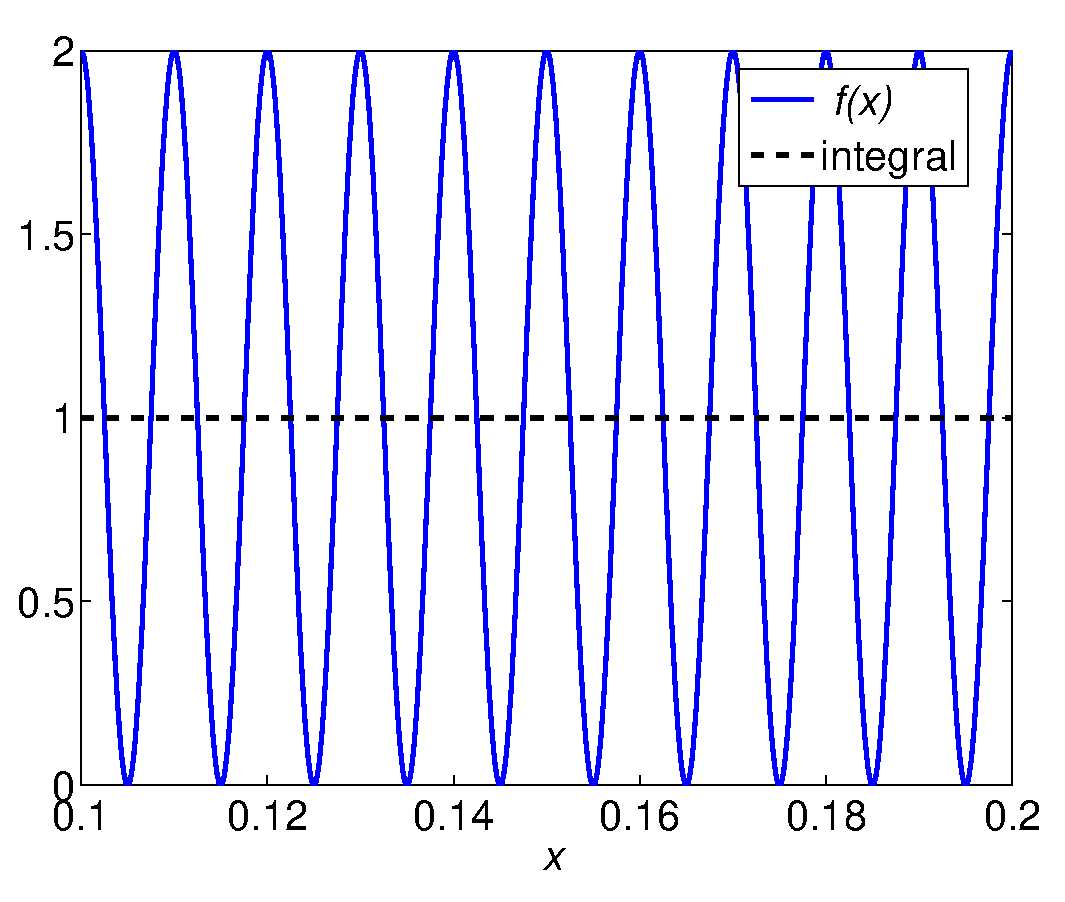
\includegraphics[width=3.7cm]{FoolQuadOscillFunctionPiece.eps}
\tabularnewline[-3ex]
\centering 
\begin{multline*}
\frac{2}{\sqrt{\pi}}\int_0^1 \me^{-x^2} \, \dif x \\
=0.8427007929497149
\end{multline*}
&
\begin{equation*}
\int_0^1 f(x) \, \dif x =1.5436
\end{equation*}
&
\begin{equation*}
\int_0^1 [1+\cos(200\pi x)] \, \dif x =1
\end{equation*}
\tabularnewline[-3ex]
\alert{\tt quad} $\to$ \newline 
{\tt 0.8427007929497149}
in {\tt 0.160521} seconds.
&
\alert{but {\tt quad}} $\to$\newline 
{\tt 2} \newline
in {\tt 0.007092} seconds.
&
\alert{but {\tt quad}} $\to$\newline  
{\tt 0.7636784919876782}
\newline in {\tt 0.205272} seconds.
\end{tabular}
\end{frame}

\begin{frame}\frametitle{Can We Have a {\hge Guarantee} Like This?}
{\hge For nice integrands, {\huge $f$}, \alert{\tt \huge quad} will provide {\huge $\int_a^b f(x) \, \dif x$} with an error {\huge $\le \varepsilon$} in a reasonable amount of time, or your money back.}  

{\hge A nice integrand, {\huge $f$}, satisfies the following conditions:} 
\begin{itemize}
\item {\smallhge \ldots, i.e., \alert{\tt \large quad} won't be fooled,}

\item {\smallhge \ldots, i.e., the number of function values required is moderate.}

\end{itemize}
{\hge If {\huge $f$} is not nice (nasty), then this guarantee is void, and {\tt \huge quad} may return an incorrect answer.}

\end{frame}

\begin{frame}\frametitle{An {\hge Impractical Guarantee}}
{\hge For integrands, {\huge $f$}, satisfying {\huge $\norm[\infty]{f''} \le M$}, a trapezoidal rule with {\huge $n=\sqrt{(b-a)^3M/(12\varepsilon)}$} trapezoids will provide  {\huge $\int_a^b f(x) \, \dif x$} with an absolute error {\huge $\le \varepsilon$}.}  

\bigskip

To apply this guarantee, one must know $M$ in advance, which is impractical.  This is why \alert{\tt quad} (adaptive recursive Simpson's rule) estimates the error and \alert{adaptively} determines the number of function evaluations, $n$. 

If the algorithm works for $f$, it should normally work for $cf$.
\end{frame}

\section{My {\tt cubMC} function}

\againframe<10>{converse}

\subsection*{Guarantee the Variance Estimate}

\begin{frame}\frametitle{Guarantee the Variance}
The \alert{sample variance}, $v$ is an unbiased estimate of $\sigma^2 = \int_{\reals^d} [f(\vx) - \mu]^2 \, \rho(\vx) \, \dif \vx$.
\begin{gather*}
v = \frac {1}{n_{\sigma}-1} \sum_{i=1}^{n_{\sigma}} [f(\vX_i)- \hmu_{n_{\sigma}}]^2, \qquad \hmu_{n_{\sigma}} = \frac 1{n_{\sigma}} \sum_{i=1}^{n_{\sigma}} f(\vX_i), \qquad \vX_1, \vX_2, \ldots \text{ i.i.d.} \sim \rho \\
\quad E[v]=\sigma^2, \qquad \var(v) = \frac{\sigma^4}{n_{\sigma}} \left ( \kappa  - \frac{n_{\sigma}-3}{n_{\sigma}-1} \right), \qquad \kappa := \frac{\int_{\reals^d} [f(\vx)-\mu]^4 \, \rho(\vx) \, \dif \vx}{\sigma^4}
\end{gather*}

\alert{Cantelli's Inequality} \citep[6.1e]{LinBai10a} guarantees that an inflated sample variance bounds the variance from above with uncertainty $\talpha$, 
\[
\alert{\hsigma^2 := \fudge^2 v, \qquad \Prob(\hsigma^2 \ge \sigma^2) \ge 1 - \talpha}, \qquad \fudge>1
\]
provided that the \alert{kurtosis} of the integrand, $\kappa$, is not too large, i.e., 
\[
\kappa
\le \frac{n_{\sigma}-3}{n_{\sigma}-1} + \left(\frac{ \talpha n_{\sigma}}{1-\talpha}\right) \left(1 - \frac{1}{\fudge^2}\right)^2 =: \kappa_{\max} (\talpha,n_{\sigma},\fudge).
\]
\end{frame}

\begin{frame}\frametitle{Guarantee the Variance}
\begin{minipage}{5cm}
\begin{gather*}
\hsigma^2 = \frac {\fudge^2}{n_{\sigma}-1} \sum_{i=1}^{n_{\sigma}} [f(\vX_i)- \hmu_{n_{\sigma}}]^2, \\
\Prob(\hsigma^2 \ge \sigma^2) \ge 1 - \talpha\\
\text{if } \kappa \le \kappa_{\max} (\talpha,n_{\sigma},\fudge)
\end{gather*}
\end{minipage}
\quad
\begin{minipage}{6.5cm}
\centering 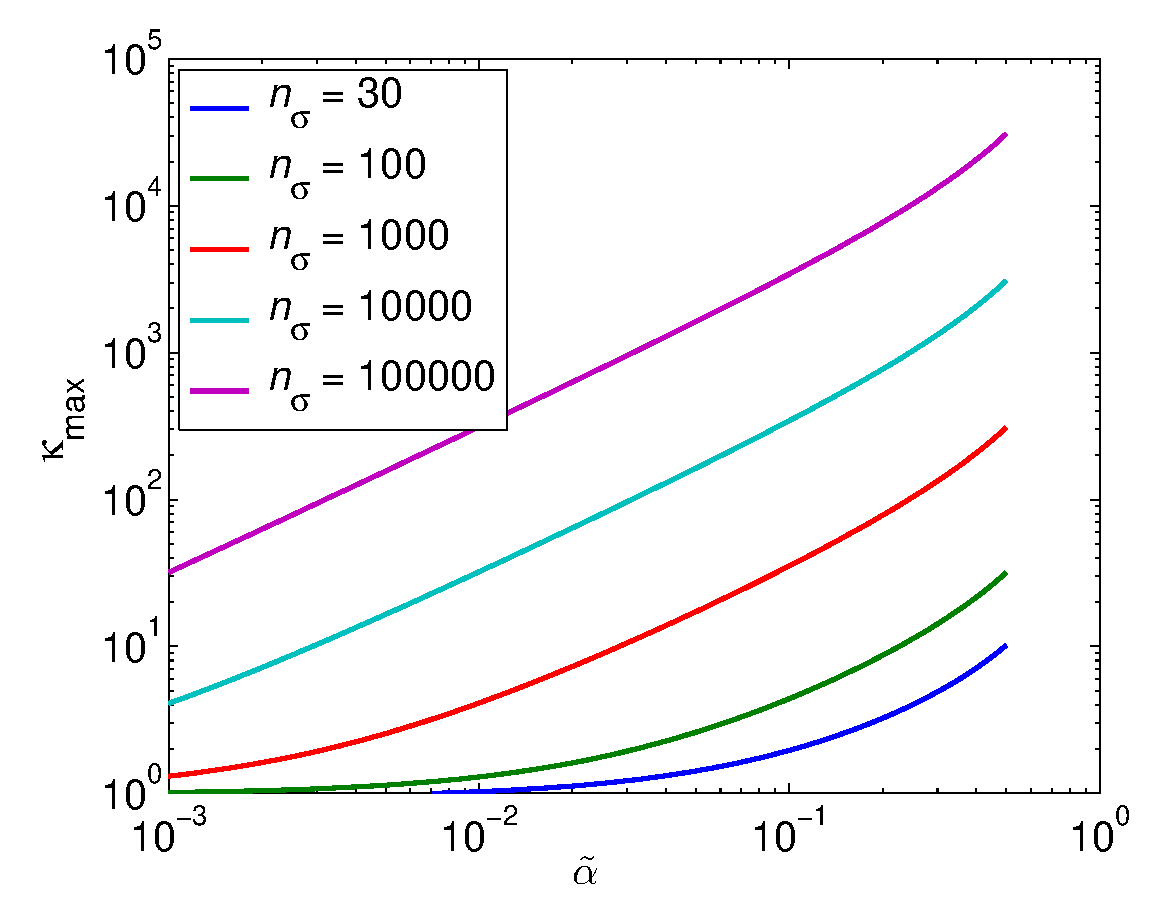
\includegraphics[width=6.5cm]{kurtmaxfig.eps}

$\fudge=1.5$
\end{minipage}
\end{frame}

\subsection*{Guarantee the Integral (Mean)}
\begin{frame}\frametitle{Guarantee the Integral (Mean)}
The \alert{Central Limit Theorem} gives an asymptotic result for fixed $z\ge 0$:
\[
\Prob\bigg[ \bigg\lvert \underbrace{\int_{\reals^d} f(\vx)\, \rho(\vx) \, \dif \vx}_\mu - \underbrace{\frac 1 n \sum_{i=1}^{n} f(\vX_{i+n_\sigma})}_{\hmu} \bigg\rvert  \le \frac{z\sigma}{\sqrt{n}} \bigg] \to 1-2\Phi(-z) \quad \text{as } n \to \infty
\]
A non-uniform \alert{Berry-Esseen Inequality} \citep[Theorem 5.16, p.\ 168]{Pet95a} gives a hard upper bound:
\begin{equation*}
\Prob\left[ \abs{\mu-\hmu}  \le \frac{z\sigma}{\sqrt{n}} \right]
\ge 1-2\left( \Phi(-z) + \alert{\frac{0.56\kappa^{3/4}}{\sqrt{n}}(1+\abs{z})^{-3}} \right)
\end{equation*}

This guarantees that $\Prob\left[ \abs{\mu-\hmu}  \le \varepsilon \right] \ge 1 - \talpha$ if the sample size is large enough:
\begin{align*}
n &\ge N_B(\varepsilon/\sigma,\talpha,\kappa) := \min \left \{ m \in \naturals : \Phi\left(-\varepsilon \sqrt{m}/\sigma  \right)+\frac{0.56 \kappa^{3/4}}{\sqrt{m}\left(1+ \varepsilon\sqrt{m}/\sigma \right)^{3}}
\le \frac{\talpha}{2} \right \}\\
& \asymp \frac{\sigma^2}{\varepsilon^2} \qquad \text{as } \frac{\varepsilon}{\sigma}\to 0
\end{align*}
\end{frame}

\begin{frame}\frametitle{{\tt cubMC}}
To evaluate $\displaystyle \mu = \int_{\reals^d} f(\vx)\, \rho(\vx) \, \dif \vx$ 

given input $f$, $\rho$, $\varepsilon$, $\alpha$, $n_{\sigma}$, $\fudge$, and $N_{\max}$:
\begin{itemize}
\item Compute $\talpha=1-\sqrt{1-\alpha}$, and the maximum kurtosis allowed, $\kappa_{\max} (\talpha,n_{\sigma},\fudge)$.  
\item Overestimate the variance: $\displaystyle \hsigma^2 = \frac {\fudge^2}{n_{\sigma}-1} \sum_{i=1}^{n_{\sigma}} [f(\vX_i)- \hmu_{n_{\sigma}}]^2$.
\item Choose the new sample size, $\displaystyle n = \min\left(\max\left(n_{\sigma}, N_B(\varepsilon/\hsigma,\talpha,\kappa_{\max}) \right),N_{\max}\right)$, for the sample mean.
\item Finally, compute the sample mean:  $\displaystyle \hmu = \frac 1 n \sum_{i=1}^{n} f(\vX_{i+n_\sigma})$.
\end{itemize}
Then $\Prob\left[ \abs{\mu-\hmu}  \le \varepsilon \right] \ge 1 - \alpha$ provided $\kappa \le \kappa_{\max}$ and $n < N_{\max}$.
\end{frame}


\subsection*{Guarantee the Cost (Sample Size, Time)}
\begin{frame}\frametitle{Guarantee the Time (Sample Size)}
Cantelli's inequality also tells us that the estimated variance, $\hsigma^2$, will not overestimate the true variance, $\sigma^2$, by much, and so the number of function values needed is not unnecessarily large:
\begin{align*}
\cost(\varepsilon,\alert{\cubMC},\sigma) & =  \sup_{f: \kappa \le \kappa_{\max}} \min_{N} \left\{ \Prob[n_{\sigma}+n \le N] \ge 1-\beta \right\}\\
&
\le n_{\sigma} + \max(n_{\sigma},N_{B}(\varepsilon/(\sigma\gamma),\talpha,\kappa_{\max}^{3/4})) \alert{\asymp \frac{\sigma^2}{\varepsilon^2}}, \\
\gamma &:= \fudge \left\{1 + \sqrt{\left(\frac{ \talpha }{1-\talpha}\right) \left(\frac{1-\beta}{\beta}\right) \left(1 - \frac{1}{\fudge^2}\right)^2}\right\}^{1/2}.
\end{align*}
\alert{Cost} depends on $\sigma^2=\var(f)$, but the algorithm \alert{does not need to know} $\sigma^2$.
\end{frame}

\begin{frame}\frametitle{{\hge Guarantee for }{\tt \huge cubMC}}
\vspace*{-4ex}
{\hge For nice integrands \alert{\tt \huge cubMC} will provide the value of {\huge $\mu = \int_{\reals^d} f(\vx) \, \rho(\vx) \, \dif \vx$} with an absolute error of {\huge $\le \varepsilon$}, with probability {\huge $1-\alpha$}, in time {\huge $\asymp (\sigma/\varepsilon)^2$} with probability {\huge $1-\beta$}, or your money back.}  

{\hge A nice integrand, {\huge $f$}, satisfies the following conditions:} 
\begin{itemize}
\item {\smallhge the kurtosis is not too large, i.e., {\large $\kappa \le \kappa_{\max} (\talpha,n_{\sigma},\fudge)$}, and}

\item {\smallhge the variance is not overwhelming, i.e., {\large $\sigma^2 \le c \varepsilon^2 N_{\max}/d$}, where {\large $N_{\max}$} is the maximum number of scalar samples.}

\end{itemize}

{\hge If {\huge $f$} is not nice (nasty), \alert{\tt \huge cubMC} may return the wrong answer.}

\end{frame}

\section{Examples and Extensions}
\subsection*{Numerical examples}
\begin{frame}\frametitle{Peak Function --- {\tt cubMC}}
\parbox{7cm}{\vspace*{-3ex}
\begin{gather*}
f(x) = \begin{cases} 
1 +  \sigma \sqrt{\frac{1-p}{p}}, & 0 \le x-z \pmod 1 \le p, \\
1 - \sigma \sqrt{\frac{p}{1-p}}, & p < x-z \pmod 1 \le 1,
\end{cases} \\
\mu = 1, \qquad \kappa = \alert{\frac{1}{p(1-p)}}-3 
\end{gather*}}
\qquad
\parbox{4cm}{\vspace*{-5ex} \centering 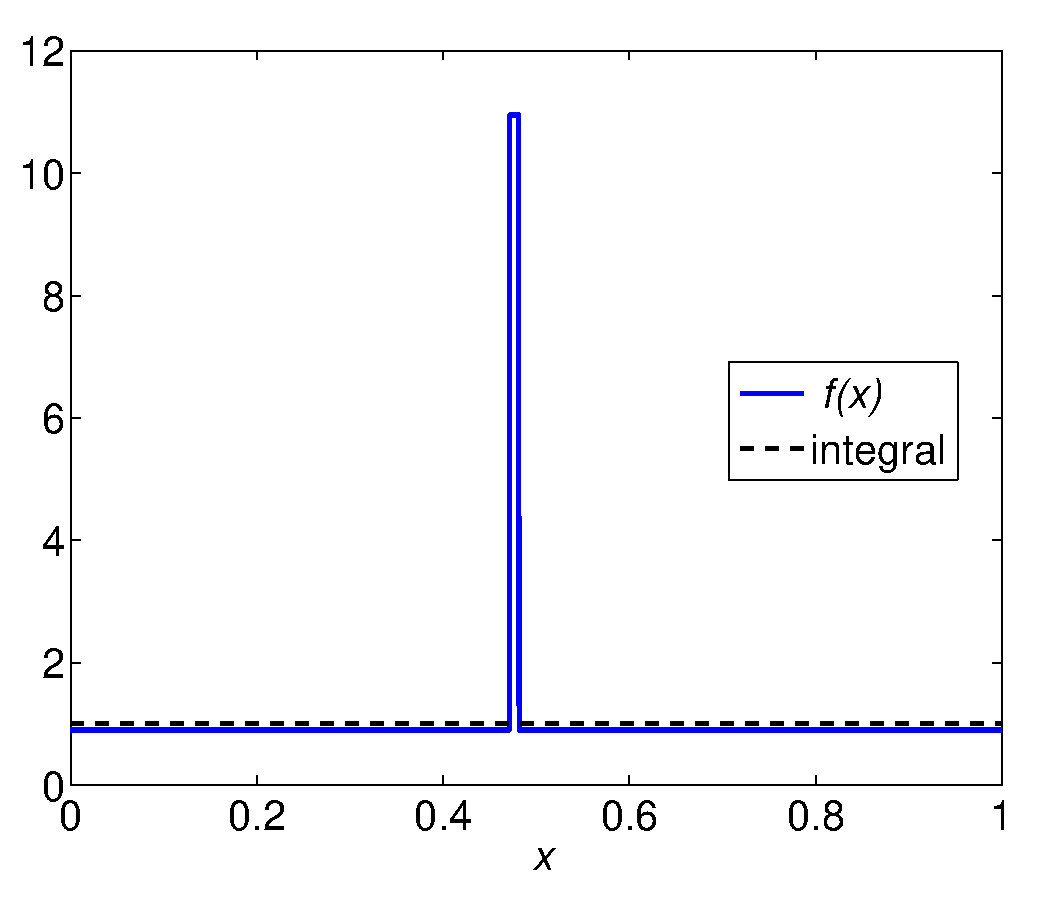
\includegraphics[width=3.5cm]{FoolQuadStepFunction.eps}}
\vspace*{-2ex}
\parbox{5cm}{
\begin{gather*}
z \sim U(0,1) \\
p\in \left[10^{-5},1/2 \right], \qquad \sigma \in \left[0.1,10 \right] \\
\log(p), \log(\sigma) \sim \text{Uniform}\\
\alpha=5\%, \qquad \fudge=1.5,\\
n_{\sigma}=1024, \qquad \alert{\varepsilon = 0.001}\\
 \kappa_{\max}=9.2, \qquad N_{\max} = 10^9\\
\text{\color{blue} covered by guarantee}\\
\text{\color{red} kurtosis too large}\\
\text{\color{brown} truncated sample}\\
\end{gather*}
}
\quad
\parbox{6cm}{\centering \includegraphics[width=6cm]{stepd=1iidErrTime.eps}}
\end{frame}

\begin{frame}\frametitle{Peak Function --- {\tt cubMC} vs.\ {\tt quad} \& {\tt quadgk}}
\begin{tabular}{>{\centering}m{4cm}>{\centering}m{4cm}@{}m{3.5cm}}
\includegraphics[width=4cm]{stepd=1iidErrTime.eps} &
\includegraphics[width=4cm]{stepd=1quadErrTime.eps} &
\[
\left\{
\begin{array}{l}
\text{MATLAB's \alert{\tt quad}} \\ 
\varepsilon = 0.001 \\
\text{fast}\\
\text{tolerance rarely met}\\
\text{\color{red} no guarantee}
\end{array}
\right .
\]
\tabularnewline
\vspace{-5ex}
\[
\begin{array}{c}
\overbrace{\text{my \alert{\tt cubMC}}} \\
\varepsilon = 0.001 \\
\text{\color{blue} covered by guarantee}\\
\text{\color{red} kurtosis too large}\\
\text{\color{brown} truncated sample}\\[5ex]
\phantom{fred}
\end{array}
\]
&
\includegraphics[width=4cm]{stepd=1quadgkErrTime.eps} &
\[
\left\{
\begin{array}{l}
\text{MATLAB's \alert{\tt quadgk}} \\ 
\varepsilon = 0.001 \\
\text{fast}\\
\text{tolerance rarely met}\\
\text{\color{red} no guarantee}
\end{array}
\right .
\]
\end{tabular}
\end{frame}

\begin{frame}\frametitle{Peak Function --- {\tt cubMC} i.i.d.\ vs.\ Sobol', Plus More Robustness}
\begin{tabular}{>{\centering}m{4cm}>{\centering}m{4cm}@{}m{3.7cm}}
\includegraphics[width=4cm]{stepd=1iidErrTime.eps} &
\includegraphics[width=4cm]{stepd=1iidheavyErrTime.eps} &
\[
\left\{
\begin{array}{l}
\text{i.i.d.\ sampling} \\ 
\text{\color{blue} covered by guarantee}\\
\text{\color{red} kurtosis too large}\\
\text{\color{brown} truncated sample}
\end{array}
\right .
\]
\tabularnewline
\includegraphics[width=4cm]{stepd=1SobolErrTime.eps} &
\includegraphics[width=4cm]{stepd=1SobolheavyErrTime.eps} &
\[
\left\{
\begin{array}{l}
\text{Sobol' sampling} \\ 
\text{\color{red} no guarantee yet \phantom{fred}}\\
\text{faster}
\end{array}
\right .
\]
\tabularnewline
$n_\sigma=1024$, $\kappa_{\max}=9.2$ & 
$n_\sigma=\alert{131072}$, $\kappa_{\max}=1050$ &
\centering $\varepsilon = 0.001$
\tabularnewline
\end{tabular}
\end{frame}

\begin{frame}\frametitle{Peak Function for $d=3$}
\begin{tabular}{>{\centering}m{4cm}>{\centering}m{4cm}@{}m{3.7cm}}
\includegraphics[width=4cm]{stepd=3iidErrTime.eps} &
\includegraphics[width=4cm]{stepd=3iidheavyErrTime.eps} &
\[
\left\{
\begin{array}{l}
\text{i.i.d.\ sampling} \\ 
\text{\color{blue} covered by guarantee}\\
\text{\color{red} kurtosis too large}\\
\text{\color{brown} truncated sample}
\end{array}
\right .
\]
\tabularnewline
\includegraphics[width=4cm]{stepd=3SobolErrTime.eps} &
\includegraphics[width=4cm]{stepd=3SobolheavyErrTime.eps} &
\[
\left\{
\begin{array}{l}
\text{Sobol' sampling} \\ 
\text{quasi-standard error} \\ 
\text{\color{red} no guarantee yet \phantom{fred}}\\
\text{faster}
\end{array}
\right .
\]
\tabularnewline
$n_\sigma=1024$, $\kappa_{\max}=9.2$ & 
$n_\sigma=\alert{131072}$, $\kappa_{\max}=1050$ &
\centering $\varepsilon = 0.001$
\tabularnewline
\end{tabular}
\end{frame}

\begin{frame}\frametitle{Asian Geometric Mean Call, $d=1, 2, 4, \ldots, 64$}
\begin{tabular}{>{\centering}m{4cm}>{\centering}m{4cm}@{}m{3.7cm}}
\includegraphics[width=4cm]{geomeaniidErrTime.eps} &
\includegraphics[width=4cm]{geomeaniidheavyErrTime.eps} &
\[
\left\{
\begin{array}{l}
\text{i.i.d.\ sampling}
\end{array}
\right .
\]
\tabularnewline
\includegraphics[width=4cm]{geomeanSobolErrTime.eps} &
\includegraphics[width=4cm]{geomeanSobolheavyErrTime.eps} &
\[
\left\{
\begin{array}{l}
\text{Sobol' sampling} 
\end{array}
\right .
\]
\tabularnewline
$n_\sigma=1024$, $\kappa_{\max}=9.2$ & 
$n_\sigma=\alert{131072}$, $\kappa_{\max}=1050$ &
\centering $\varepsilon = 0.02$
\tabularnewline
\end{tabular}
\end{frame}


\subsection*{Discussion}
\begin{frame}\frametitle{Why an Adaptive Algorithm?}
\vspace*{-3ex}
\begin{tabular}{>{\centering}p{5.8cm}>{\centering}p{5.8cm}}
\alert{\tt cubMC} & \alert{non-adaptive algorithm}\tabularnewline
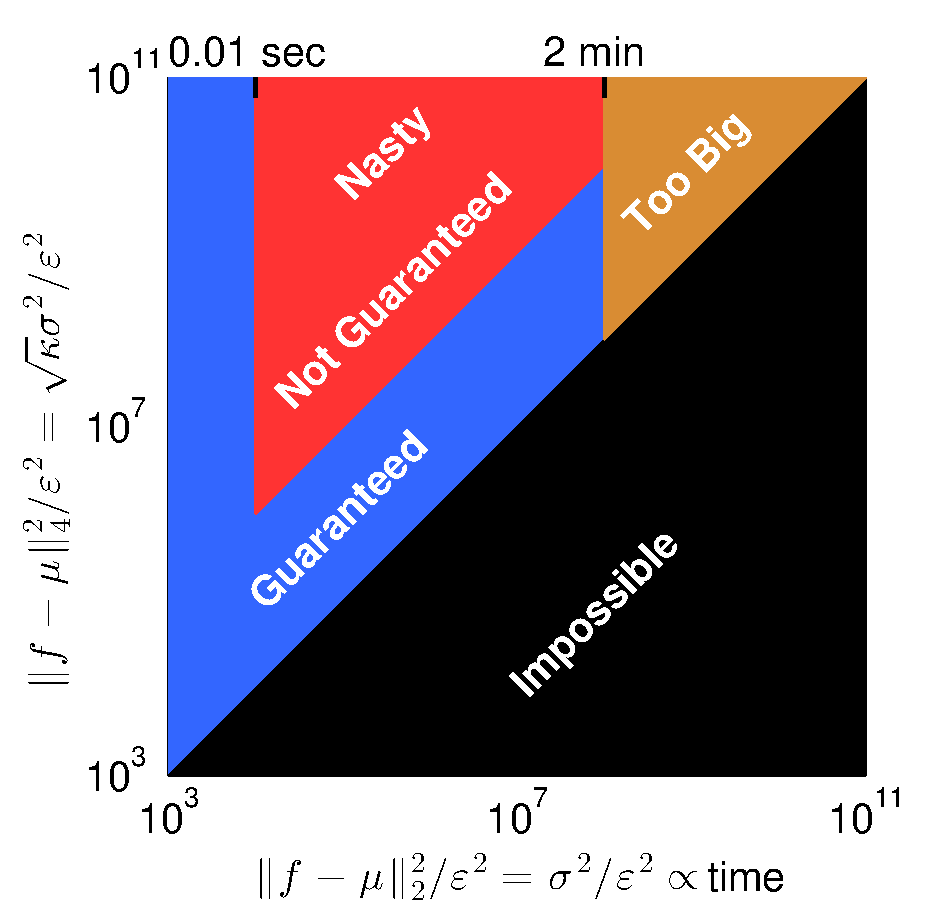
\includegraphics[width=4.8cm]{AdaptGuaranteedRegion.eps} &
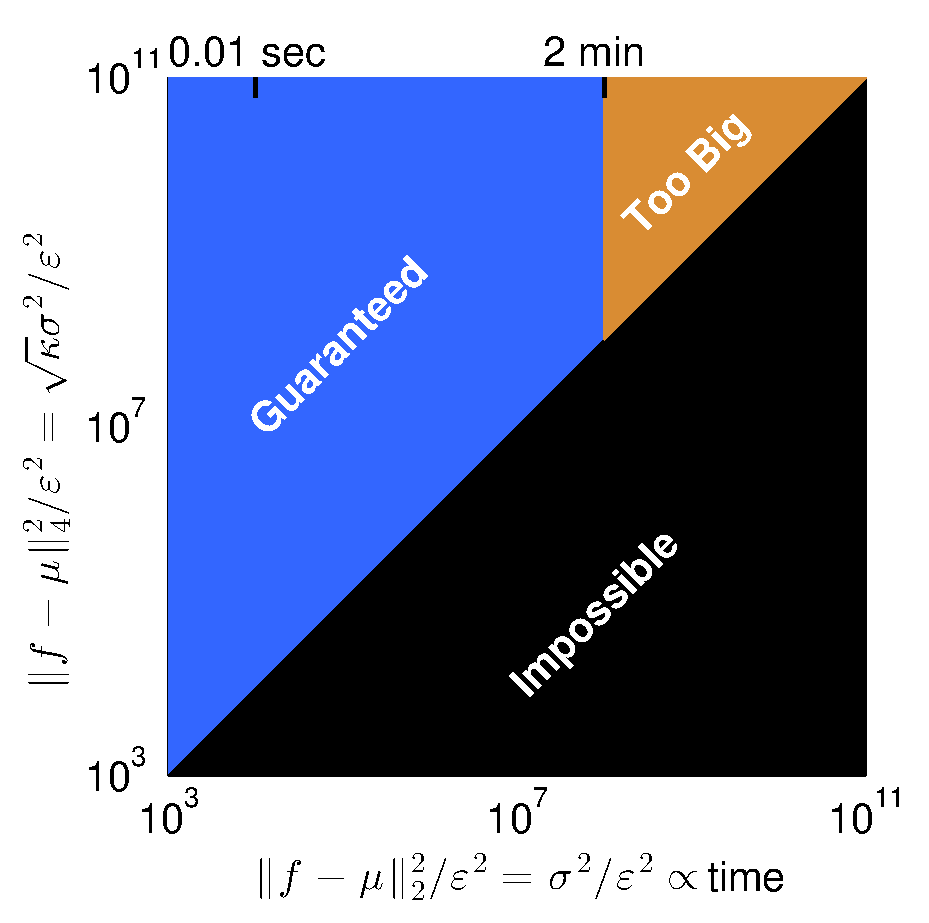
\includegraphics[width=4.8cm]{NonAdaptGuaranteedRegion.eps}\tabularnewline[-2ex]
\begin{itemize}
\item Cost depends on size of integrand 
\item Algorithm parameters determine robustness to nasty integrands
\item Tiny integrands handled regardless
\item Huge integrands cannot be handled
\end{itemize}
&
\begin{itemize}
\item Cost is fixed and high if you want it reach tolerance for lots of integrands 
\item Huge integrands cannot be handled
\end{itemize}
\end{tabular}
\end{frame}

\begin{frame}[label=whykurt]\frametitle{Why Make {\tt cubMC} Dependent on Kurtosis?}
\centerline{\framebox[1.1\width]{$\sigma = $\alert{ difficulty} \qquad $\kappa = $\alert{ nastiness}}}

\bigskip

The kurtosis of a random variable or function, 
\[
\kappa = \frac{E[(Y-\mu)^4]}{\underbrace{\{E[(Y-\mu)^2]\}^2}_{\sigma^4}} \quad \text{or} \quad \kappa := \frac{\displaystyle\int_{\reals^d} [f(\vx)-\mu]^4 \, \rho(\vx) \, \dif \vx}{\underbrace{\left\{\int_{\reals^d} [f(\vx)-\mu]^2 \, \rho(\vx) \, \dif \vx\right\}^2}_{\sigma^4}}
\]
is difficult to estimate.  Why should \alert{\tt cubMC}'s guarantee depend on bounded  $\kappa$?
\begin{itemize}
\item Practically, we need $\kappa$ bounded to justify the estimates of $\sigma^2$.
\item Bounded $\kappa$ yields sets of probability distributions or functions that are \alert{non-convex}.  
\begin{itemize}
\item Nonparametric confidence intervals are \alert{impossible} for \alert{convex} sets of distributions \citep[Corollary 2]{BahSav56}. \hfill\hyperlink{nonconvexdist}{\beamergotobutton{How we break convexity}}
\item \alert{Adaptive information does not help} for \alert{convex} sets of integrands in the worst case and probabilistic settings \citep[Chapter 4, Theorem 5.2.1; Chapter 8, Corollary 5.3.1]{TraWasWoz88}.
\hfill\hyperlink{nonconvexfun}{\beamergotobutton{How we break convexity}}
\end{itemize}
\end{itemize}
\end{frame}

\begin{frame}[label=qse]\frametitle{Quasi-Standard Error (Internal Replications) for Quasi-Random Sequences}
Let $\vX_1, \vX_2, \ldots$ be a (random or deterministic) sequence, let $r$ be fixed, and let 
\[
\hmu_m=\frac{1}{2^m} \sum_{i=1}^{2^m} f(\vX_i) = \frac{1}{2^r} \sum_{j=1}^{2^r} \hmu_{m,j}, \qquad \hmu_{m,j}=\frac{1}{2^{m-r}} \sum_{i=1}^{2^{m-r}} f(\vX_{(j-1)2^{m-r}+i})
\]
The \alert{quasi-standard error} \citep{Owe97} measures the variation of among the means of parts of the whole sample
\[
\qse_m=\sqrt{\frac{1}{2^r(2^r-1)} \sum_{j=1}^{2^r} (\hmu_{m,j}-\hmu_m)^2}
\]

Given error tolerance, $\varepsilon$, and parameters $r\in \naturals$, $m_1\ge r$, and $\fudge > 1$, for $m=m_1, m_1+1, \ldots$,
\begin{itemize}
\item  Compute $f(\vX_{2^{m-1}+1}), \ldots, f(\vX_{2^{m}})$, and $\hmu_{m,1}, \ldots, \hmu_{m,2^r}, \hmu_m$.

\item If $\fudge\qse_m \le \varepsilon$, then stop.  Else continue.
\end{itemize}
\hfill\hfill\hyperlink{whyqse}{\beamergotobutton{When this works}}
\end{frame}



\subsection*{Summary \& Further Work}
\begin{frame}[label=FurtherWork]\frametitle{Further Work}
\begin{description}

\item[Quasi-Monte Carlo Sampling] --- What is a good measure of an integrand being nasty or nice?

\item[Variance Reduction Techniques] --- Can we preserve the guarantee?

\item[Different Error Criteria] --- Worst case? Randomized?

\item[Lower Bounds on Cost] --- The typical fooling functions are nasty (high kurtosis).  Does assuming moderate kurtosis make the problem easier?

\item[Relative Error Tolerances] --- Both the variance and the mean are needed to determine the eventual sample size.

\item[Unbounded or Infinite $d$] --- Can automatic integrators for finite $d$ be used in multilevel methods to improve efficiency? \hfill\hfill\hyperlink{timedim}{\beamergotobutton{Look here}}

\item[Other Problems] --- Are there any guarantees for MATLAB's \alert{\tt quad}, or any other univariate adaptive quadrature routine that estimates error?  What about guarantees for function approximation?

\end{description}
\end{frame}

\part{References}
\frame[allowframebreaks]{\frametitle{References}
\bibliographystyle{spbasic}
\bibliography{FJH22,FJHown22}
}

\section{Extra Material}
\subsection*{Breaking Convexity}
\begin{frame}[label=nonconvexdist]\frametitle{A Set of Distributions with Bounded Kurtosis is Non-Convex}
\begin{tabular}{>{\centering}m{5.7cm}>{\centering}m{5.7cm}}
\begin{gather*}
\Prob(Y_1 = y) = 0.5, \ y=\pm 1 \\
\Prob(Y_2 = y) = 0.5, \ y=\pm 2 \\
f_{3} =  \frac 12 f_{1} + \frac 12 f_{2}\\
\Prob(Y_3 = y)= 0.25, \ y=\pm 1, \pm 2\\
\kappa_3 = \alert{\frac{34}{25} > 1} =\kappa_1=\kappa_2
\end{gather*}
&
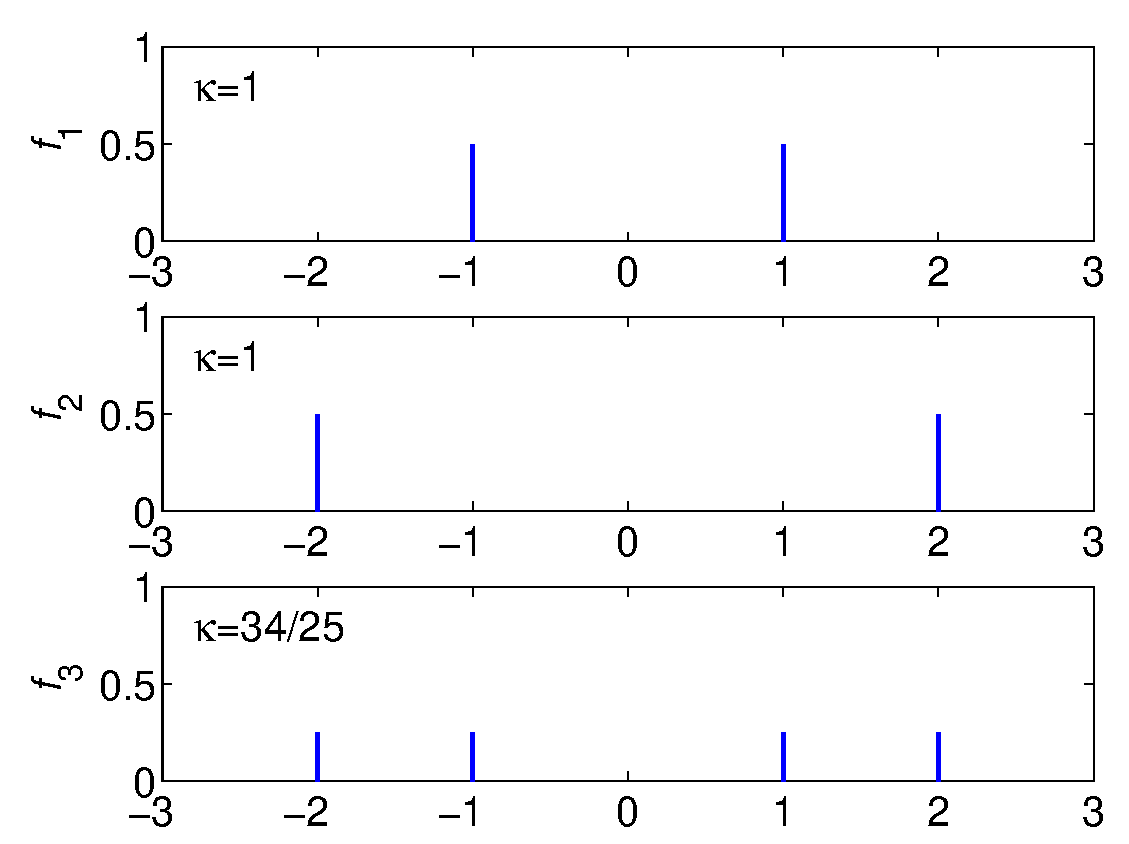
\includegraphics[width=5.5cm]{ConvexSumDist.eps}
\end{tabular}

\hfill \hfill\hyperlink{whykurt}{\beamerreturnbutton{Return}}
\end{frame}

\begin{frame}[label=nonconvexfun]\frametitle{A Set of Integrands with Bounded Kurtosis is Non-Convex}

\begin{tabular}{>{\centering}m{5.7cm}>{\centering}m{5.5cm}}
\[
\begin{array}{rl}
f_1(x) & = \begin{cases} 
-1, 
& 0 \le x < 1/2\\
1, & 1/2 \le x \le 1 
\end{cases} \\[4ex]
f_2(x) &= 
\begin{cases} 1, & 0 \le x < 1/4\\
-1, & 1/4 \le x \le 3/4 \\
 1, & 3/4 \le x \le 1
\end{cases} \\[7ex]
f_3(x) &= \frac 12 f_1(x) + \frac 12 f_2(x) \\
&= \begin{cases} 
0, & 0 \le x < 1/4,\\
-1, & 1/4 \le x \le 1/2, \\
0, & 1/2 \le x \le 3/4, \\
 1, & 3/4 \le x \le 1,
\end{cases}\\[7ex]
\kappa_3=\alert{2} &\alert{> 1}= \kappa_1=\kappa_2
\end{array}
\]
&
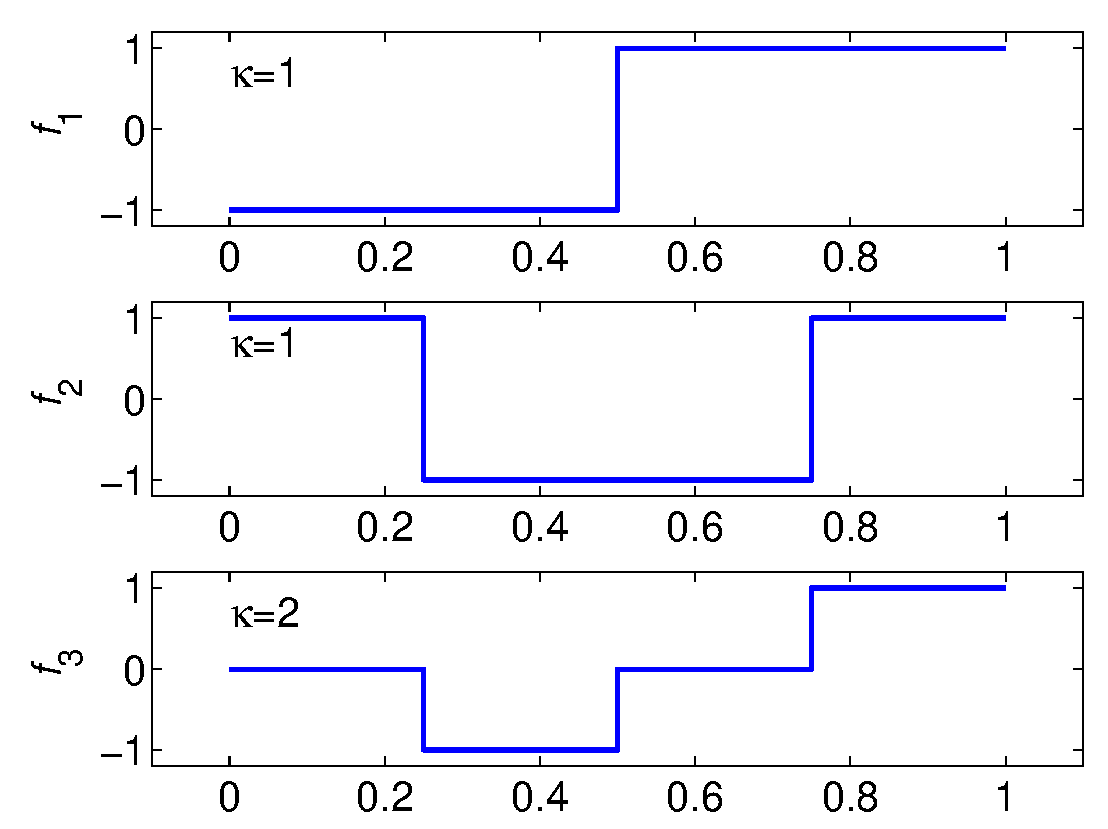
\includegraphics[width=5.5cm]{ConvexSumFun.eps}

\bigskip

\hfill \hfill\hyperlink{whykurt}{\beamerreturnbutton{Return}}
\end{tabular}
\end{frame}

\subsection*{When Quasi-Standard Error Works}
\begin{frame}[label=whyqse]\frametitle{When Does Quasi-Standard Error Work?}
Quasi-standard error has been proposed by Warnock and studied by \cite{Owe97,Sny00a,Hal05a,Owe06a}. Suppose that $\vX_1, \vX_2, \ldots$ is a scrambled digital $(t,d)$-sequence in base $2$, $P_{m}=\{\vX_1, \ldots, \vX_{2^{m}}\}$, and the integrand can be expanded in a Walsh series:
\begin{gather*}
f(\vx) = \sum_{\vk \in \naturals_0^d} \hf(\vk) \me^{\pi \sqrt{-1} \vk \otimes \vx}, \qquad (S_{B}f)(\vx) := \sum_{\vk \in B} \hf(\vk) \me^{\pi \sqrt{-1} \vk \otimes \vx} \quad\text{(filtered $f$)}\\
\mu = \int_{[0,1)^d} f(\vx) \, \dif \vx = S_{\{\vzero\}}f, \qquad \hmu_m=\frac{1}{2^m} \sum_{i=1}^{2^m} f(\vX_i) = (S_{P_m^{\perp}}f)(\vX_1),
\end{gather*}
where $\otimes$ is a bitwise dot product modulo 2, and $P_m^{\perp}=\{\vk \in \naturals_0^d : \vk \otimes \vx = 0 \ \forall \vx \in P_m\}$ is the \alert{dual net} (wavenumbers aliased with $\vzero$).
The \alert{quasi-standard error} may be expressed as
\[
\qse_m=\sqrt{\frac{1}{2^r-1} \sum_{\vl \in (P_{m-r}^{\perp}/P_m^{\perp}) \setminus \{\vzero\}} (S_{P_m^{\perp}\oplus \vl}f)^2(\vX_1) }
\]
which is a surrogate for $\abs{\mu - \hmu_m} = \abs{(S_{P_m^{\perp}\setminus\{\vzero\}}f)(\vX_1)}$.

\end{frame}


\begin{frame}\frametitle{When Does Quasi-Standard Error Work?}
\begin{minipage}{6cm}
\begin{gather*}
f(\vx) = \sum_{\vk \in \naturals_0^d} \hf(\vk) \me^{\pi \sqrt{-1} \vk \otimes \vx}\\
%\mu = \int_{[0,1)^d} f(\vx) \, \dif \vx = S_{\{\vzero\}}f\\
%\hmu_m=\frac{1}{2^m} \sum_{i=1}^{2^m} f(\vX_i) = (S_{P_m^{\perp}}f)(\vX_1)\\
\abs{\mu - \hmu_m} = \abs{(S_{P_m^{\perp}\setminus\{\vzero\}}f)(\vX_1)} \quad \only<1>{{\color{red}\bullet} P_6^{\perp}\setminus\{\vzero\}}
\only<2>{{\color{red}\bullet} P_7^{\perp}\setminus\{\vzero\}}
\only<3>{{\color{red}\bullet} P_8^{\perp}\setminus\{\vzero\}}
\only<4>{{\color{red}\bullet} P_9^{\perp}\setminus\{\vzero\}}
\only<5>{{\color{red}\bullet} P_{10}^{\perp}\setminus\{\vzero\}}
\end{gather*}
\end{minipage}
\quad
\begin{minipage}{5.5cm}
\centering
\only<1>{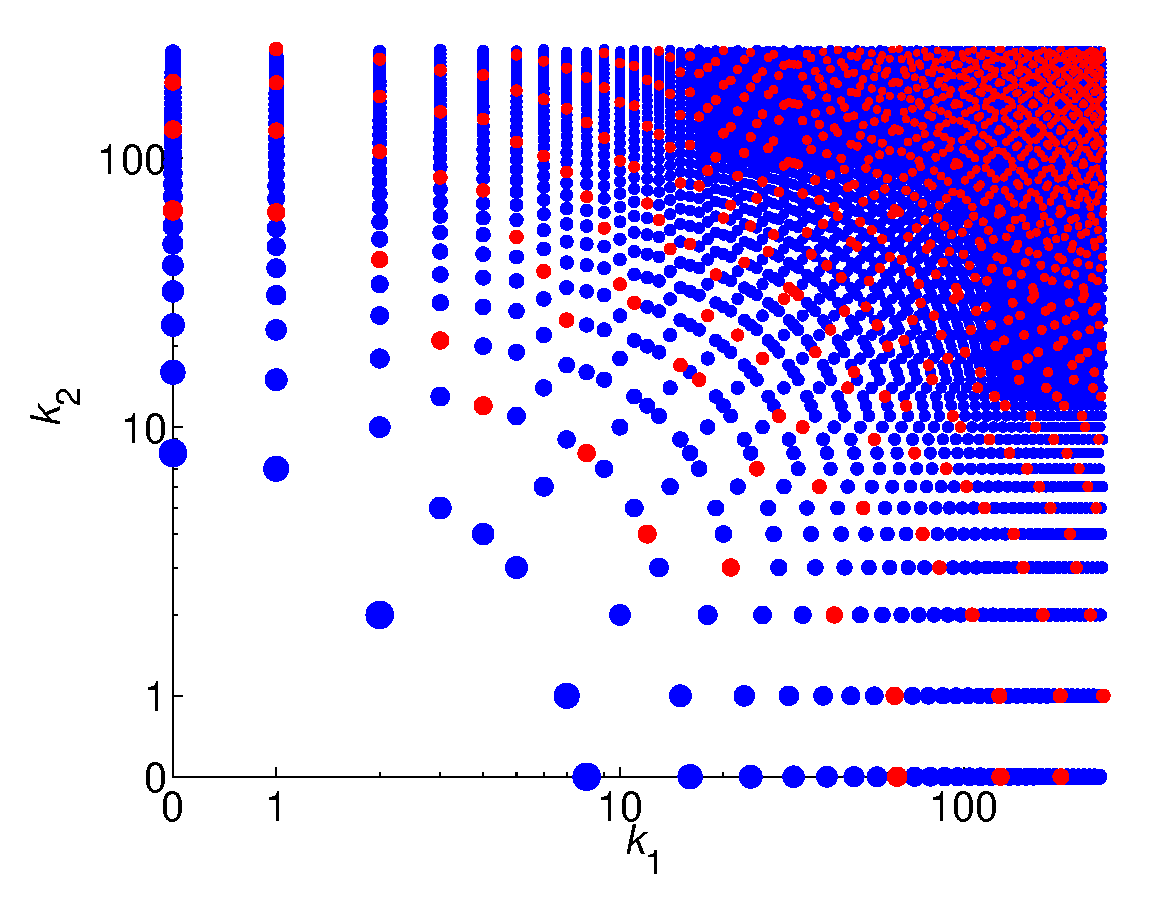
\includegraphics[width=5.5cm]{dualnet-6.eps}
%\\ {\color{red}$\bullet$} $P_6^{\perp}\setminus\{\vzero\}$\qquad{\color{blue}$\bullet$} $P_{3}^{\perp}\setminus P_{6}^{\perp}$
}
\only<2>{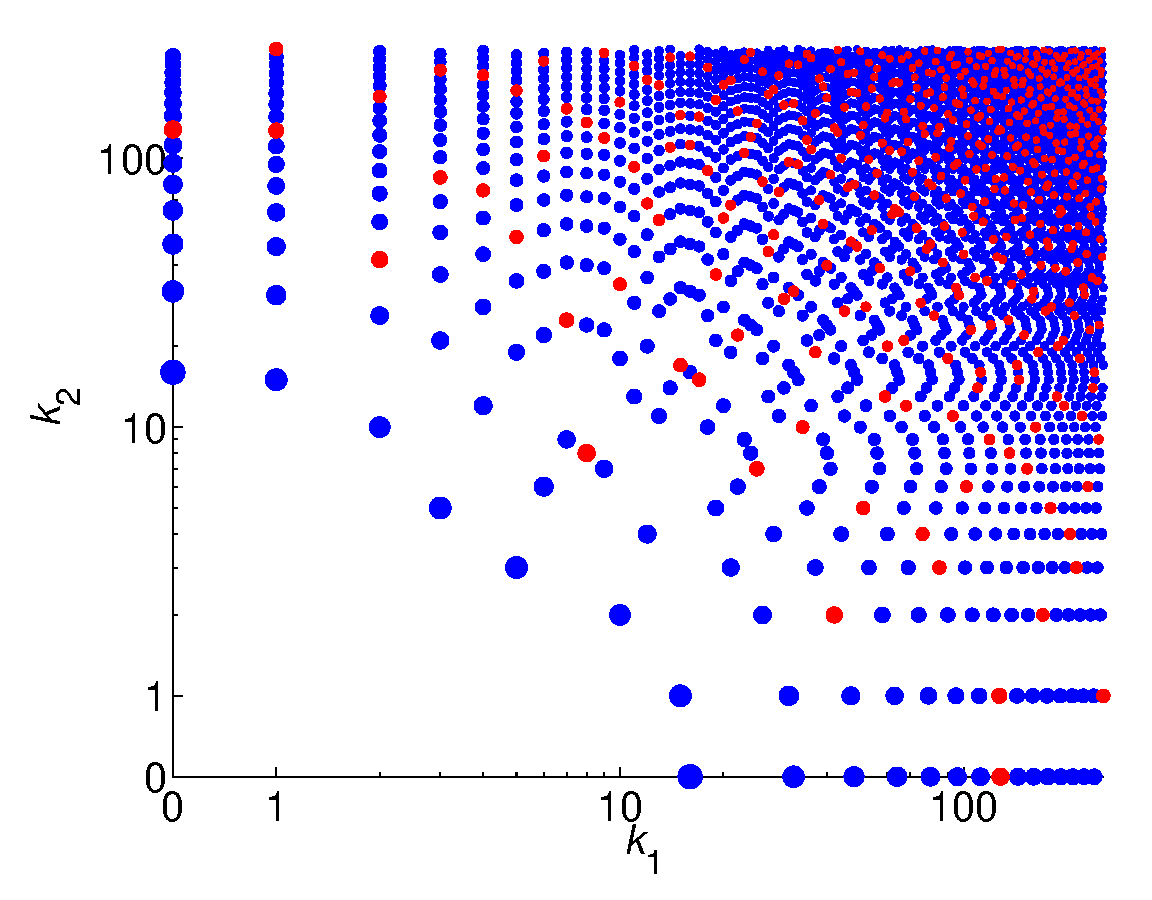
\includegraphics[width=5.5cm]{dualnet-7.eps}
%\\{\color{red}$\bullet$} $P_7^{\perp}\setminus\{\vzero\}$\qquad{\color{blue}$\bullet$} $P_{4}^{\perp}\setminus P_{7}^{\perp}$
}
\only<3>{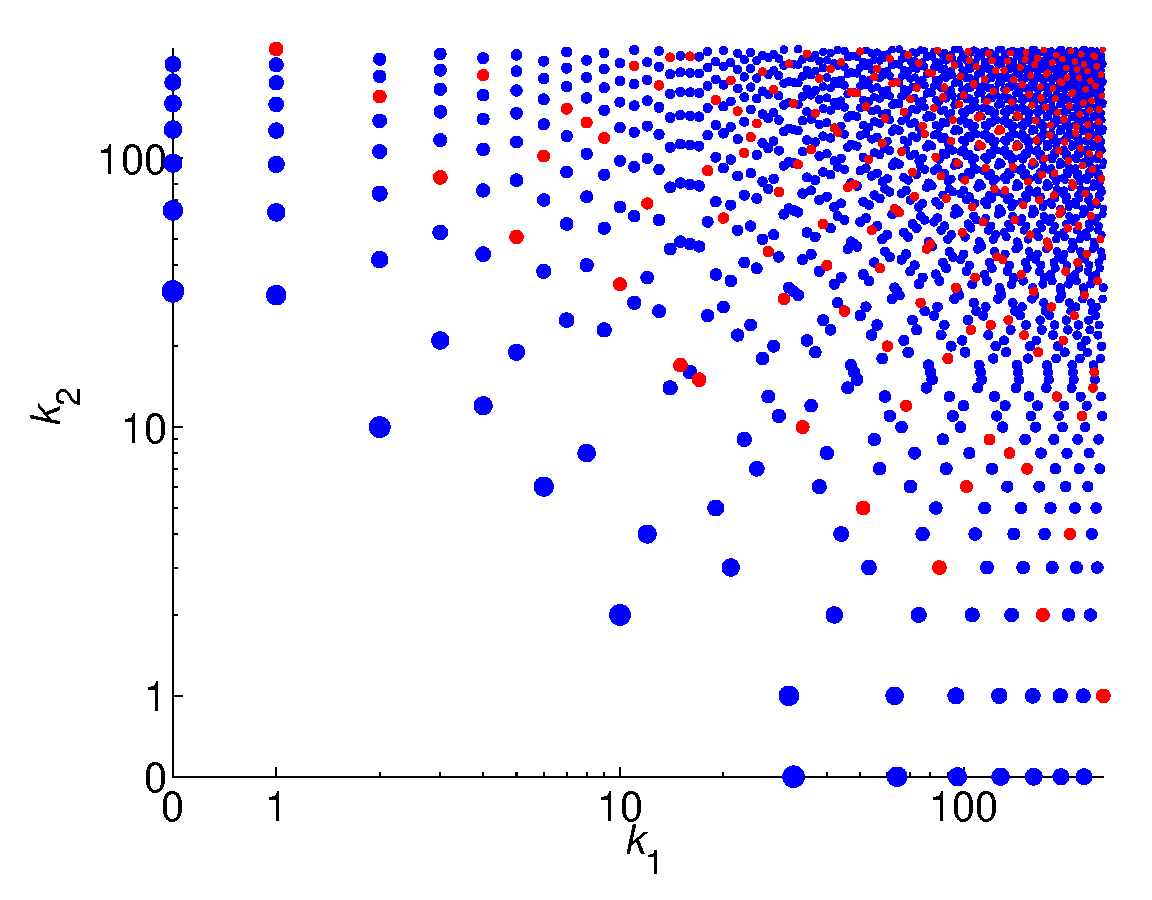
\includegraphics[width=5.5cm]{dualnet-8.eps}
%\\{\color{red}$\bullet$} $P_8^{\perp}\setminus\{\vzero\}$\qquad{\color{blue}$\bullet$} $P_{5}^{\perp}\setminus P_{8}^{\perp}$
}
\only<4>{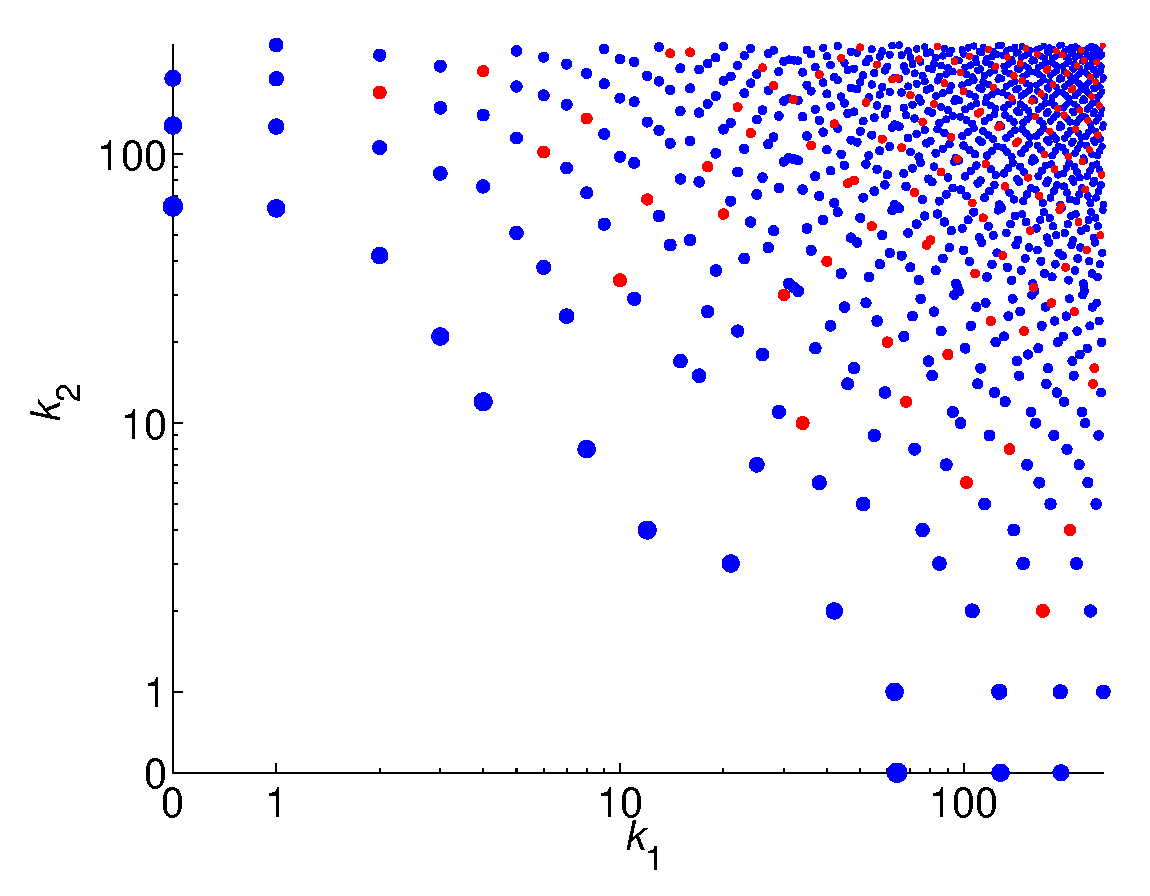
\includegraphics[width=5.5cm]{dualnet-9.eps}
%\\{\color{red}$\bullet$} $P_9^{\perp}\setminus\{\vzero\}$\qquad{\color{blue}$\bullet$} $P_{6}^{\perp}\setminus P_{9}^{\perp}$
}
\only<5>{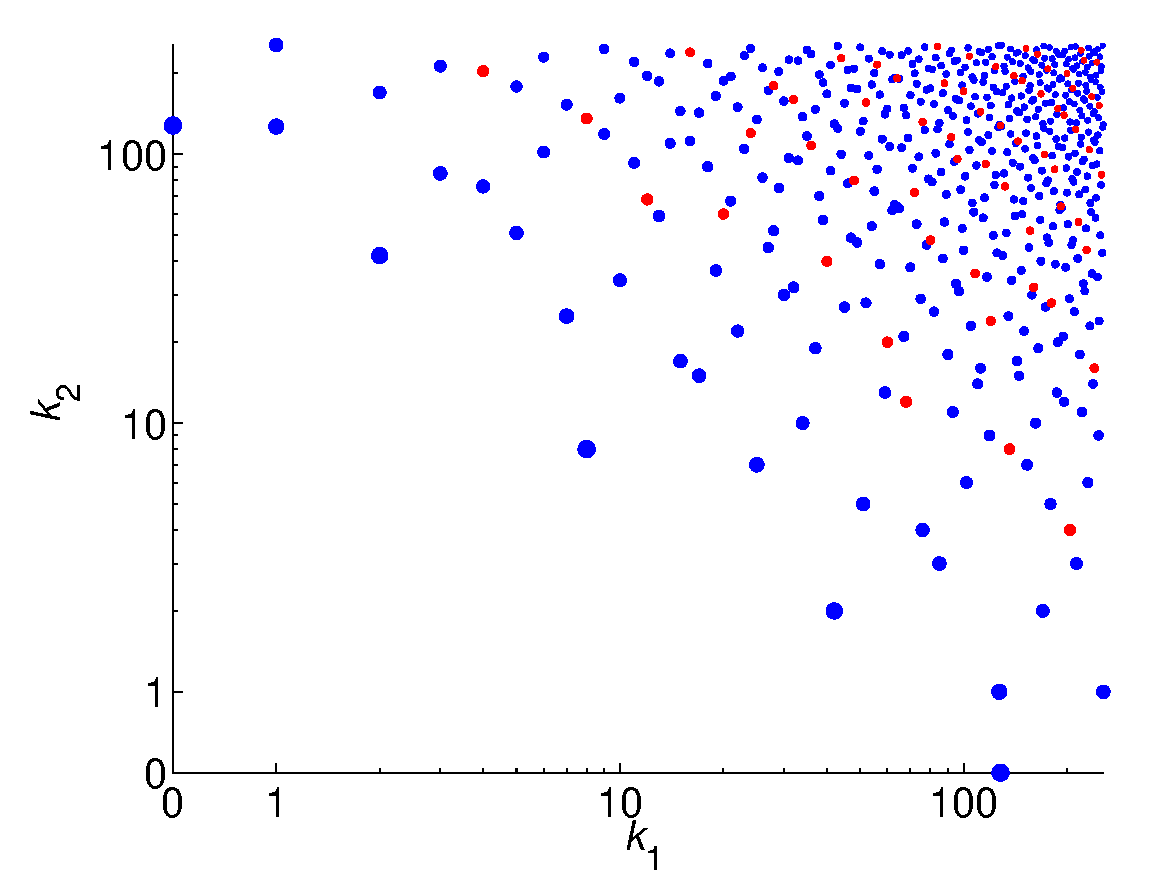
\includegraphics[width=5.5cm]{dualnet-10.eps}
%\\{\color{red}$\bullet$} $P_{10}^{\perp}\setminus\{\vzero\}$\qquad{\color{blue}$\bullet$} $P_{7}^{\perp}\setminus P_{10}^{\perp}$
}
\end{minipage}
\[
\qse_m=\sqrt{\frac{1}{7} \sum_{\vl \in (P_{m-3}^{\perp}/P_m^{\perp}) \setminus \{\vzero\}} (S_{P_m^{\perp}\oplus \vl}f)^2(\vX_1) } \qquad 
\only<1>{{\color{blue}\bullet} P_{3}^{\perp}\setminus P_{6}^{\perp}}
\only<2>{{\color{blue}\bullet} P_{4}^{\perp}\setminus P_{7}^{\perp}}
\only<3>{{\color{blue}\bullet} P_{5}^{\perp}\setminus P_{8}^{\perp}}
\only<4>{{\color{blue}\bullet} P_{6}^{\perp}\setminus P_{9}^{\perp}}
\only<5>{{\color{blue}\bullet} P_{7}^{\perp}\setminus P_{10}^{\perp}}
\]
\hfill \hfill\hyperlink{qse}{\beamerreturnbutton{Return}}
\end{frame}

\begin{frame}[label=timedim]\frametitle{Asian Geometric Mean Call Execution Times}
\begin{tabular}{>{\centering}m{4cm}>{\centering}m{4cm}@{}m{3.7cm}}
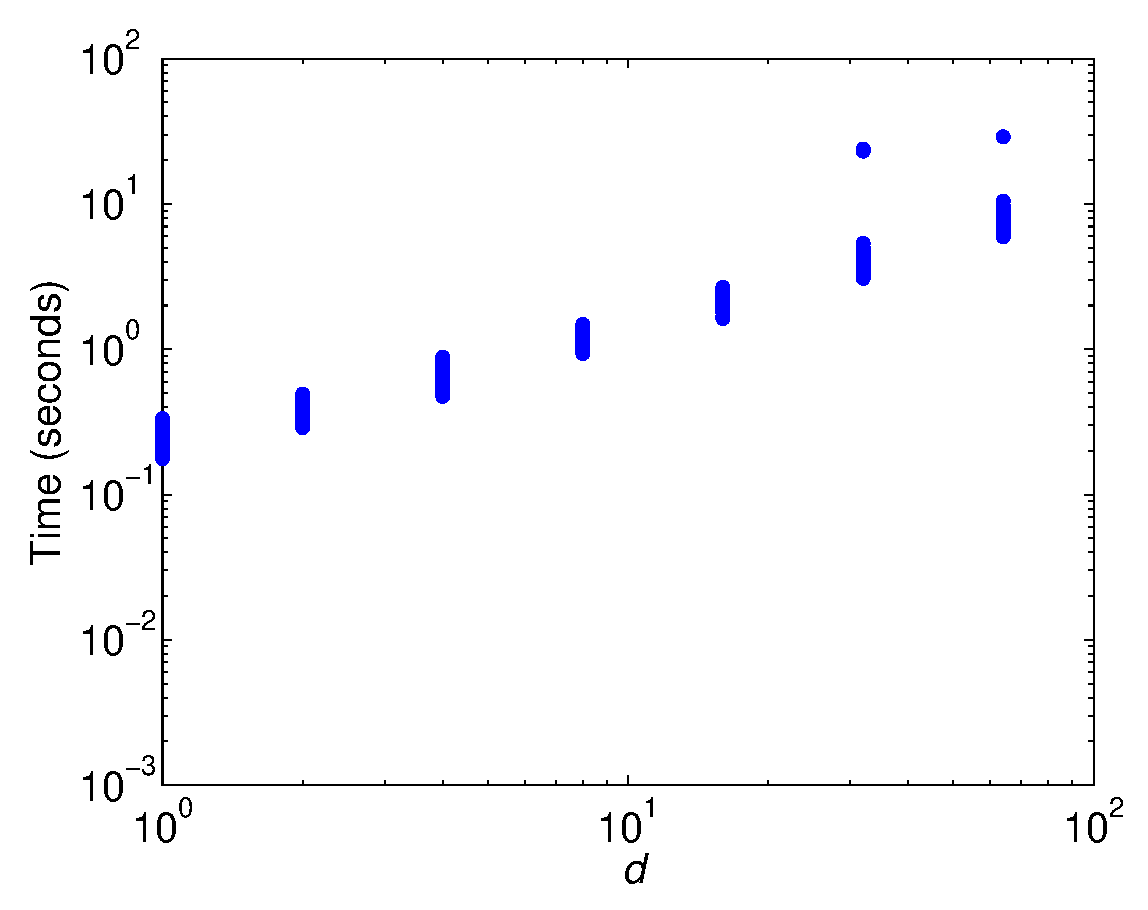
\includegraphics[width=4cm]{iidtimedim.eps} &
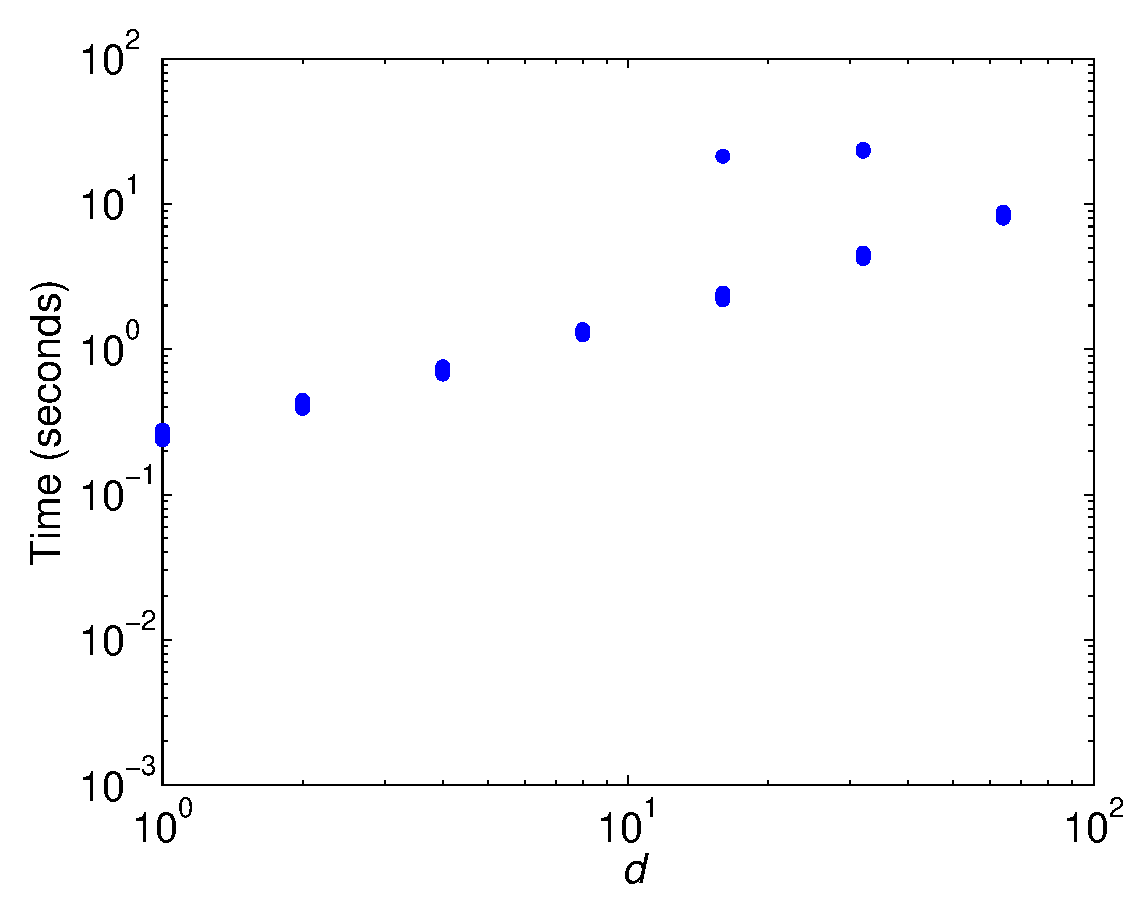
\includegraphics[width=4cm]{iidheavytimedim.eps} &
\[
\left\{
\begin{array}{l}
\text{i.i.d.\ sampling}
\end{array}
\right .
\]
\tabularnewline
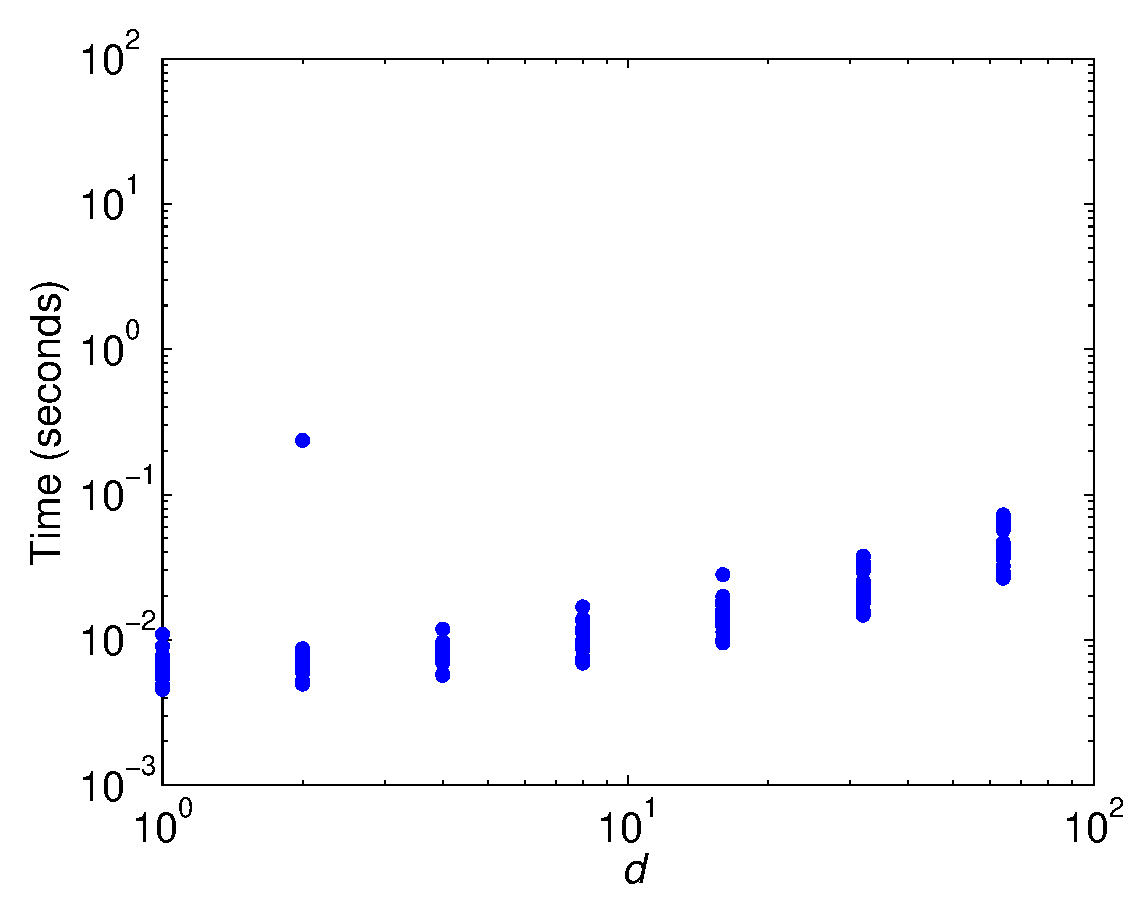
\includegraphics[width=4cm]{Soboltimedim.eps} &
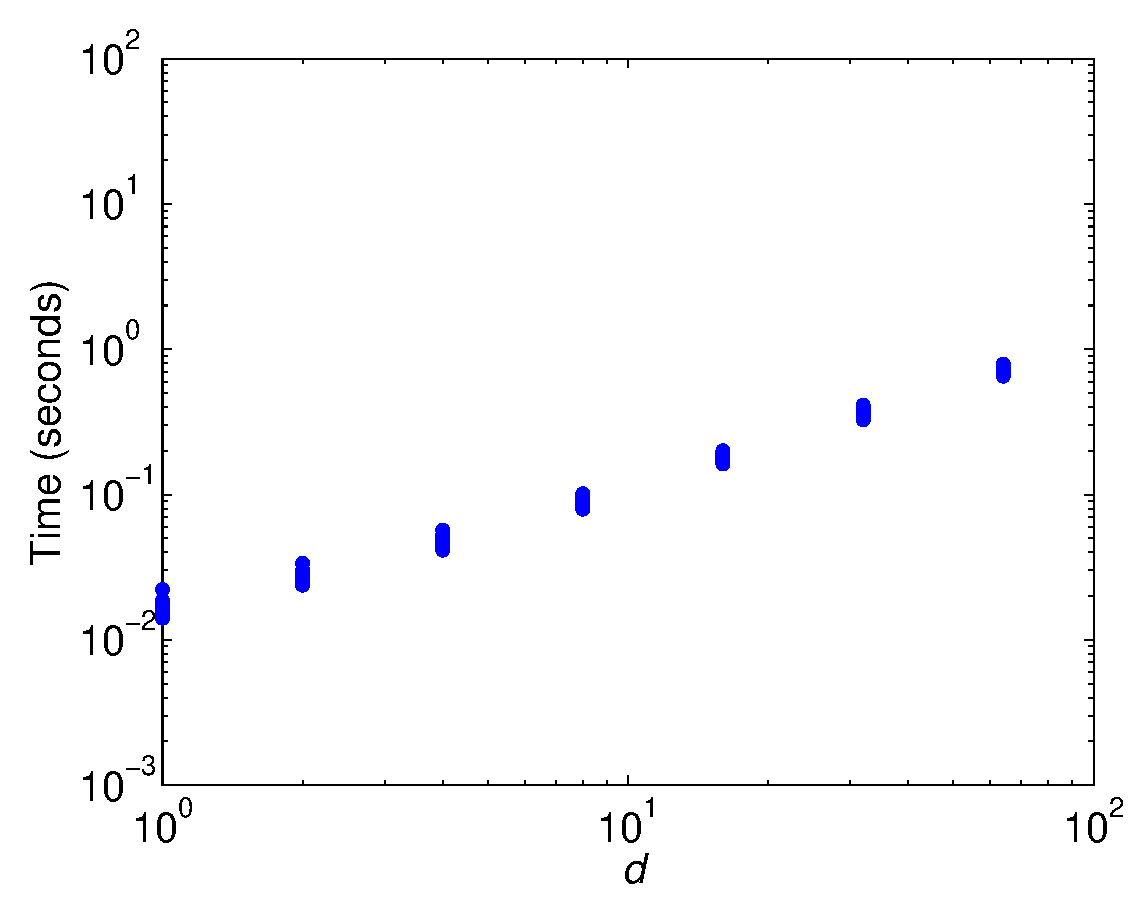
\includegraphics[width=4cm]{Sobolheavytimedim.eps} &
\[
\left\{
\begin{array}{l}
\text{Sobol' sampling} 
\end{array}
\right .
\]
\tabularnewline
$n_\sigma=1024$, $\kappa_{\max}=9.2$ & 
$n_\sigma=\alert{131072}$, $\kappa_{\max}=1050$ &
\hfill \hfill\hyperlink{FurtherWork}{\beamerreturnbutton{Return}}
\tabularnewline
\end{tabular}
\end{frame}



\end{document}


\begin{frame}\frametitle{Peak Function --- {\tt cubMC} with More Robustness}
\begin{tabular}{>{\centering}b{5.7cm}>{\centering}b{5.7cm}}
my \alert{\tt cubMC} with i.i.d.\ sampling, $\varepsilon = 0.001$\linebreak $n_\sigma=1024$, $\kappa_{\max}=9.2$ & 
my \alert{\tt cubMC} with i.i.d.\ sampling, $\varepsilon = 0.001$ \linebreak $n_\sigma=\alert{131072}$, $\kappa_{\max}=1050$ \tabularnewline
\includegraphics[width=5.8cm]{stepd=1iidErrTime.eps} &
\includegraphics[width=5.8cm]{stepiidheavyErrTime.eps} \tabularnewline
\text{\color{blue} covered by guarantee}\linebreak
\text{\color{red} kurtosis too large}\linebreak
\text{\color{brown} truncated sample} &
\text{\color{blue} covered by guarantee}\linebreak
\text{\color{red} kurtosis too large}\linebreak
\text{\color{brown} truncated sample}
\end{tabular}
\end{frame}

\begin{frame}\frametitle{Peak Function --- {\tt cubMC} with Sobol' and More Robustness}
\begin{tabular}{>{\centering}b{5.7cm}>{\centering}b{5.7cm}}
my \alert{\tt cubMC} with Sobol' sampling, $\varepsilon = 0.001$\linebreak $n_\sigma=1024$& 
my \alert{\tt cubMC} with Sobol' sampling, $\varepsilon = 0.001$ \linebreak $n_\sigma=\alert{131072}$ \tabularnewline
\includegraphics[width=5.8cm]{stepSobolErrTime.eps} &
\includegraphics[width=5.8cm]{stepSobolheavyErrTime.eps} \tabularnewline
\text{\color{blue} covered by guarantee}\linebreak
\text{\color{red} kurtosis too large}\linebreak
\text{\color{brown} truncated sample} &
\text{\color{blue} covered by guarantee}\linebreak
\text{\color{red} kurtosis too large}\linebreak
\text{\color{brown} truncated sample}
\end{tabular}
\end{frame}

\begin{frame}\frametitle{Peak Function --- {\tt cubMC} --- i.i.d.\ vs.\ Sobol' Sampling}
\begin{tabular}{>{\centering}b{5.7cm}>{\centering}b{5.7cm}}
my \alert{\tt cubMC} with i.i.d.\ sampling \linebreak $\varepsilon = 0.001$ &
my \alert{\tt cubMC} with Sobol' sampling \linebreak $\varepsilon = 0.001$ \tabularnewline 
\includegraphics[width=5.7cm]{stepd=1iidErrTime.eps} &
\includegraphics[width=5.7cm]{stepd=1SobolErrTime.eps}\tabularnewline
\text{\color{blue} covered by guarantee}\linebreak
\text{\color{red} kurtosis too large}\linebreak
\text{\color{brown} truncated sample} &
faster\linebreak
meets tolerance similarly\linebreak
\text{\color{red} no guarantee yet}
\end{tabular}
\end{frame}





